\section{Numerical Experiments}
%We provide numerical evidence supporting our conclusions.


\subsection{Simulating Theorem \ref{thm:char}}\label{subsec:lemma_sims}
In the proof of Theorem \ref{thm:char} we utilize Lemma
\ref{lemma:free} to construct D-optimal designs. We implement this
construction with the goal of testing numerically how prevalent are
clustered designs. We iterate over the number of measurements $m \in
\{4,\dots, 24\}$, and for every $m$ we then iterate over $k:=\rank
\obs^*\obs \in \{2,\dots, m-1\}$. For each pair $m,k$ we run $N=5000$
simulations according to the following steps:
\begin{enumerate}
\item Generate random diagonal $D\in \mathbb{R}^{k\times k}$ with
  entries $\log (d_i) \sim \mathcal{N}(25,15)$ and normalize it so
  that $\ttr D = m$.
\item Conjugate $D$ by a random orthogonal matrix to form a positive
  semi-definite $M := UDU^t \in \mathbb{R}^{k\times k}$.
\item Apply the construction of Lemma \ref{lemma:free} to calculate
  $A$ such that $AA^t = M$, where $A$ has unit norm columns.
\item Since columns of $A$ correspond to measurement vectors, we call
  $A$ "clustered" if $A$ has two or more identical columns (up to some
  numerical precision threshold).
\end{enumerate}
We then calculate the fraction of clustered designs of the simulations
we ran, for each pair $m,k$. Clusterization occurred at high rates
($>99.9\%$) whenever $m-k > 1$; see Fig.~\ref{fig:sim_AAt}. Hence, in
these simulations, clusterization is a generic property. However, when
$m-k = 1$, clusterization does not occur. We do not why and further
investigation into this phenomenon is out of scope for the current
study.

\begin{figure}
    \centering
    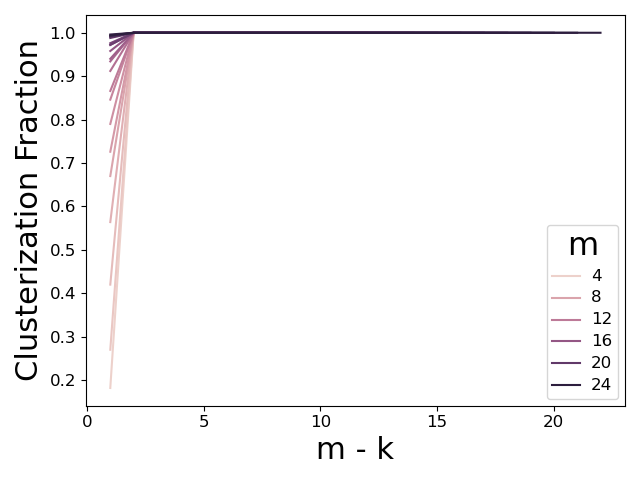
\includegraphics[height=0.5\textwidth]{figs/simulations.png}
    \caption{Fraction of clustered $A$ for $AA^t = M$ and $M$
      generated randomly (see text and repository for details on
      generating $M$). It is evident that when $m-k \geq 2$ clusterization
      is ubiquitous, whereas for lower $m-k$ clusterization does not
      occur.}
  \label{fig:sim_AAt}
\end{figure}

Full results are located in the \texttt{simulations.csv} file within
the accompanying \href{https://github.com/yairdaon/OED}{repository},
code implementing the experiments described above is located in module
\texttt{zeros.py} of said repository.


\subsection{Correlated errors}\label{subsec:corr_errors_sims}
In order to verify the results of Section \ref{section:non_vanishing},
we run simulations of the inverse problem of the 1D heat equation with
nonvanishing model error \(\modcov = \prcov^2 \). Indeed, including
model correlation pushes measurements apart, see
Fig.~\ref{fig:corr_errors}. Code generating Fig.~\ref{fig:corr_errors}
is located in module \texttt{clusterization.py} in the accompanying
\href{https://github.com/yairdaon/OED}{repository}.

\begin{figure}
    \centering
    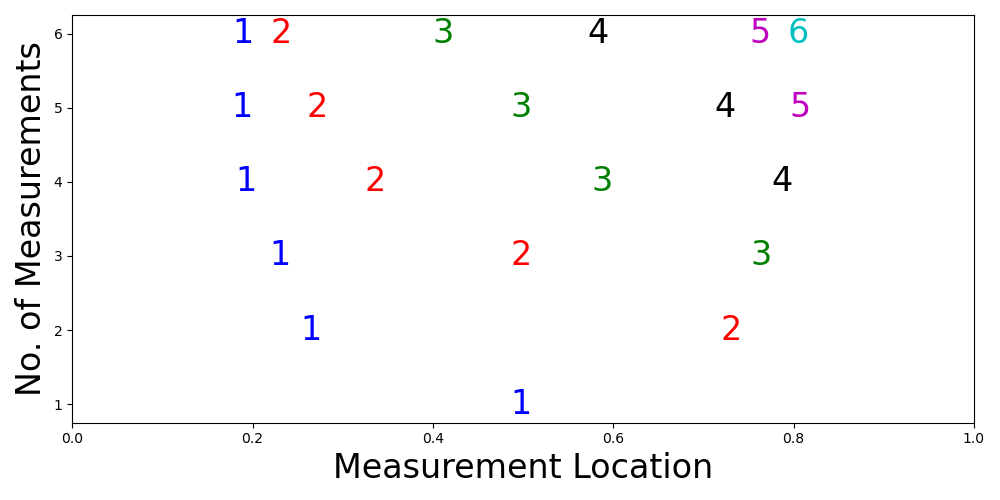
\includegraphics[height=0.5\textwidth]{figs/dst_modelError4.png}
    \caption{Model correlation mitigates clusterization. We add a
      model correlation term to the error terms in the 1D heat
      equation inverse problem. Lo and behold, measurements are not
      close anymore and are pushed away thanks to the model error
      term.}
  \label{fig:corr_errors}
\end{figure}

%% \subsection{Implementing the 1D heat equation}
%% The Laplacian $\Delta$ is a Fourier multiplier \cite{stein2009}, so
%% our implementation proceeds in frequency space. When we utilize the
%% homogeneuous Dirichlet boundary condition, the eigenvectors of
%% $\Delta$ are sines $\ev_n(x) = \sin(\pi n x), n=1,2,3,\dots$, whereas
%% for the homogenoeous Neumann boundary condition the eigenvectors are
%% cosines $\cos(\pi n x)$. Implementing point evaluations in Fourier
%% space

